\chapter{\emph{Image Enhancement} (melhoramento) no domínio da frequência}

Capítulo 4 de Gonzalez, \textit{Digital Image Processing}~\cite{gonzalez2006image}.

\noindent
Seção 7 de Ramirez, \textit{The FFT: Fundamentals and Concepts}~\cite{ramirez1975fft}.

%%%%%%%%%%%%%%%%%%%%%%%%%%%%%%%%%%%%%%%%%%%%%%%%%%%%%%%%%%%%
\section{Introdução}

\begin{easylist}

  & Transformada de Fourier é uma maneira de representar um sinal como uma integral de senos e cossenos multiplicados por uma função de peso. Um sinal pode ser convertido para sua representação transformada e reconvertido de volta para o domínio original sem perda de informação. Também é possível realizar operações como filtragens na representação transformada e reconverter de volta para o domínio original.

\end{easylist}
  
%%%%%%%%%%%%%%%%%%%%%%%%%%%%%%%%%%%%%%%%%%%%%%%%%%%%%%%%%%%%
\section{A transformada de Fourier}

\begin{easylist}

  & Transformada de Fourier $g(u)$ de uma função contínua de uma única variável é dada pela fórmula

  \[ g(u) = \int^{\infty}_{-\infty} f(x) e^{-j2\pi ux} dx \]

  onde $j = \sqrt{-1}$, De maneira análoga, dado $g(u)$, podemos obter $f(x)$ através da transformada inversa de Fourier
  
  \[ f(x) = \int^{\infty}_{-\infty} g(u) e^{ j2\pi ux} du \]

\vspace{1cm}
  
  & Essas operações possuem uma versão para duas variáveis

  \[ g(u, v) = \int^{\infty}_{-\infty}\int^{\infty}_{-\infty} f(x, y) e^{-j2\pi (ux + vy)} dx dy \]

  e sua inversa

  \[ f(x, y) = \int^{\infty}_{-\infty}\int^{\infty}_{-\infty} g(u, v) e^{ j2\pi (ux + vy)} dx dy \]

  & Muitas vezes é mais fácil manipular as versões contínuas da transformada de Fourier, mas para trabalhar com imagens, usamos suas versões discretas

  \[ g(u) = \frac 1M \sum^{M-1}_{x=0} f(x) e^{-j2\pi ux/M} \textrm{para u de 0 a $M-1$} \]

  e sua inversa

  \[ f(x) =          \sum^{M-1}_{u=0} g(u) e^{ j2\pi ux/M} \textrm{para x de 0 a $M-1$} \]

  & O conceito de domínio da frequência segue a fórmula de Euler

  \[ e^{j\theta} = \cos\theta + j\sin\theta \]

  & Substituindo na transformada direta discreta, temos

  \[ g(u) = \frac 1M \sum^{M-1}_{x=0} f(x) (\cos (2\pi ux/M) -j\sin (2\pi ux/M)) \]

  & e na transformada inversa discreta, temos

  \[ f(x) = \sum^{M-1}_{u=0} g(u) (\cos (2\pi ux/M) +j\sin (2\pi ux/M)) \]

  & A transformada de Fourier discreta bidimensional pode ser calculada pela fórmula

  \[ g(u, v) = \frac 1{MN} \sum^{M-1}_{x=0}\sum^{N-1}_{y=0} f(x, y) e^{-j2\pi (ux/M + vy/N)} \].

  Nesse caso, a inversa pode ser calculada pela fórmula

  \[ f(x, y) =             \sum^{M-1}_{x=0}\sum^{N-1}_{y=0} g(u, v) e^{ j2\pi (ux/M + vy/N)} \].

\clearpage
  
  & Substituindo a fórmula de Euler na transformada discreta bidimensional de Fourier, obtemos

  \[ g(u, v) = \frac 1{MN} \sum^{M-1}_{x=0}\sum^{N-1}_{y=0} f(x, y)
      \cos\left(2\pi \left(\frac{ux}{M} + \frac{vy}{N}\right)\right) -
     j\sin\left(2\pi \left(\frac{ux}{M} + \frac{vy}{N}\right)\right)   \]

  e sua inversa

  \[ f(x, y) =             \sum^{M-1}_{x=0}\sum^{N-1}_{y=0} g(u, v)
      \cos\left(2\pi \left(\frac{ux}{M} + \frac{vy}{N}\right)\right) +
     j\sin\left(2\pi \left(\frac{ux}{M} + \frac{vy}{N}\right)\right)   \]

\end{easylist}
  
%%%%%%%%%%%%%%%%%%%%%%%%%%%%%%%%%%%%%%%%%%%%%%%%%%%%%%%%%%%%
\section{\textit{Fast Fourier Transform}}

\begin{easylist}

  & A complexidade do algoritmo da transformada de Fourier é quadrática no número de pixels da imagem. Para calcular cada pixel da imagem de saída, é necessário consultar todos os pixels da imagem de entrada. Se $P$ é o número de pixels da imagem, a complexidade da transformada de Fourier é $O(P^2)$. Felizmente, é possível acelerar o cálculo através do uso da Fast Fourier Transform (FFT), cuja complexidade é $O(P\log(P))$. A seguir veremos o algoritmo de Sande-Tukey descrito por Ramirez~\cite{ramirez1975fft}.

  & O algoritmo requer como entrada um vetor unidimensional cujo tamanho é uma potência de 2. Para processar imagens bidimensionais, é necessário primeiro aplicar o algoritmo em todas as linhas da imagem de entrada, e em seguida, em todas as colunas da imagem resultante.

  & A expressão para calcular a DFT de um sinal unidimensional é dada por

  \[ g(u) = \frac 1M \sum^{M-1}_{x=0} f(x) e^{-j2\pi ux/M} \]

para u de 0 a $M-1$.
  
  & Seja $W = e^{-j2\pi/M}$. Omitindo o fator $1/M$, que pode ser aplicado no final do cálculo, e trocando $f$ por $f_0$, onde o índice subscrito denota o estágio do cálculo, teremos

  \[ g(u) = \sum^{M-1}_{x=0} f_0(x) W^{-ux} \].

\begin{figure}[!b]
  \begin{center}
    \begin{tabular}{c}
      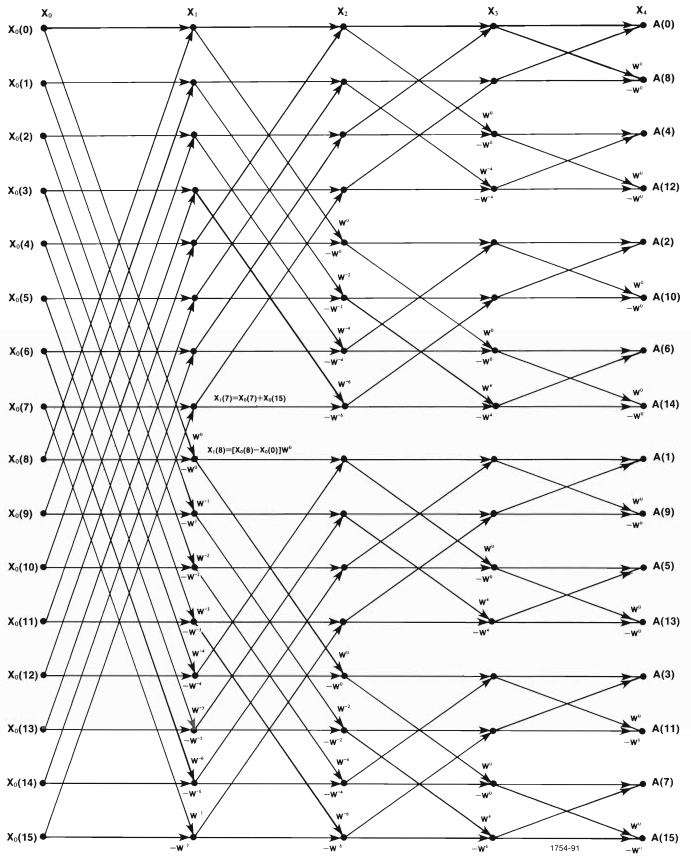
\includegraphics[width=1\textwidth]{images/04/fft.png}
    \end{tabular}
  \end{center}
  \caption{\label{fig:fft} Esquema de uma FFT de um vetor de tamanho 16.}
\end{figure}


\clearpage
  
  & O cálculo da FFT consiste de $\log_2 M = K$ estágios. Cada estágio requer pares de cálculos da forma

  \[ f_{k+1}(r) = f_k(r) + f_k(s) \]

  e

  \[ f_{k+1}(s) = (f_k(r) + f_k(s)) W^{-p} \]

  para inteiros $r, s, p$ entre 0 e $M-1$, e para $k$ de 0 a $K$.

  & A Figura~\ref{fig:fft} mostra o esquema do cálculo da FFT de um vetor de tamanho $M = 16$. Cada conjunto de 4 setas saindo de um par $(f_k(r), f_k(s))$ e chegando em um par $(f_{k+1}(r), f_{k+1}(s))$, pelo seu formato, é chamado \textit{butterfly}.

  & A diferença entre $s$ e $r$ diminui com o aumento de $k$ e é dada por $2^{K-k-1}$. Já o expoente $p$ começa sempre como 0 em cada grupo de \textit{butterflies} que se sobrepõem. O incremento do valor de $p$ depende de $k$ e é dado por $2^{k+1}$. A tabela~\ref{tab:fft} mostra os cálculos necessários para obter a FFT de um vetor de tamanho $M = 16$.

\end{easylist}

\begin{table}[!h]
  \centering
  \begin{tabular}{|l|l|l|}
      \hline
      $k=0$ & $k=1$  \\
      $s-r=8$ & $s-r=4$  \\
      $\Delta p = 1$ & $\Delta p = 2$  \\
      \hline
      $f_1(0 ) = (f_0(0 ) + f_0(8 ))      $ & $f_2(0)  = (f_1(0 ) + f_1(4 ))      $  \\
      $f_1(1 ) = (f_0(1 ) + f_0(9 ))      $ & $f_2(1)  = (f_1(1 ) + f_1(5 ))      $  \\
      $f_1(2 ) = (f_0(2 ) + f_0(10))      $ & $f_2(2)  = (f_1(2 ) + f_1(6 ))      $  \\
      $f_1(3 ) = (f_0(3 ) + f_0(11))      $ & $f_2(3)  = (f_1(3 ) + f_1(7 ))      $  \\
      $f_1(4 ) = (f_0(4 ) + f_0(12))      $ & $f_2(4)  = (f_1(0 ) - f_1(4 )) W^{-0}$  \\
      $f_1(5 ) = (f_0(5 ) + f_0(13))      $ & $f_2(5)  = (f_1(1 ) - f_1(5 )) W^{-2}$  \\
      $f_1(6 ) = (f_0(6 ) + f_0(14))      $ & $f_2(6)  = (f_1(2 ) - f_1(6 )) W^{-4}$  \\
      $f_1(7 ) = (f_0(7 ) + f_0(15))      $ & $f_2(7)  = (f_1(3 ) - f_1(7 )) W^{-6}$  \\
      $f_1(8 ) = (f_0(0 ) - f_0(8 )) W^{-0}$ & $f_2(8)  = (f_1(8 ) + f_1(12))       $  \\
      $f_1(9 ) = (f_0(1 ) - f_0(9 )) W^{-1}$ & $f_2(9)  = (f_1(9 ) + f_1(13))       $  \\
      $f_1(10) = (f_0(2 ) - f_0(10)) W^{-2}$ & $f_2(10) = (f_1(10) + f_1(14))       $  \\
      $f_1(11) = (f_0(3 ) - f_0(11)) W^{-3}$ & $f_2(11) = (f_1(11) + f_1(15))       $  \\
      $f_1(12) = (f_0(4 ) - f_0(12)) W^{-4}$ & $f_2(12) = (f_1(8 ) - f_1(12)) W^{-0} $  \\
      $f_1(13) = (f_0(5 ) - f_0(13)) W^{-5}$ & $f_2(13) = (f_1(9 ) - f_1(13)) W^{-2} $  \\
      $f_1(14) = (f_0(6 ) - f_0(14)) W^{-6}$ & $f_2(14) = (f_1(10) - f_1(14)) W^{-4} $  \\
      $f_1(15) = (f_0(7 ) - f_0(15)) W^{-7}$ & $f_2(15) = (f_1(11) - f_1(15)) W^{-6} $  \\
      \hline
      \hline
      $k=2$ & $k=3$  \\
      $s-r=2$ & $s-r=1$  \\
      $\Delta p = 4$ & $\Delta p = 8$  \\
      \hline
      $f_3(0 ) = (f_2(0 ) + f_2(2 ))      $ & $f_4(0 ) = (f_3(0 ) + f_3(1 ))      $  \\
      $f_3(1 ) = (f_2(1 ) + f_2(9 ))      $ & $f_4(1 ) = (f_3(0 ) - f_3(1 )) W^{-0}$  \\
      $f_3(2 ) = (f_2(0 ) - f_2(2 )) W^{-0}$ & $f_4(2 ) = (f_3(2 ) + f_3(3 ))      $  \\
      $f_3(3 ) = (f_2(1 ) - f_2(3 )) W^{-4}$ & $f_4(3 ) = (f_3(2 ) - f_3(3 )) W^{-0}$  \\
      $f_3(4 ) = (f_2(4 ) + f_2(6 ))      $ & $f_4(4 ) = (f_3(4 ) + f_3(5 ))      $  \\
      $f_3(5 ) = (f_0(5 ) + f_0(7 ))      $ & $f_4(5 ) = (f_3(4 ) - f_3(5 )) W^{-0}$  \\
      $f_3(6 ) = (f_2(4 ) - f_2(6 )) W^{-0}$ & $f_4(6 ) = (f_3(6 ) + f_3(7 ))      $  \\
      $f_3(7 ) = (f_2(5 ) - f_2(7 )) W^{-4}$ & $f_4(7 ) = (f_3(6 ) - f_3(7 )) W^{-0}$  \\
      $f_3(8 ) = (f_2(8 ) + f_2(10))      $ & $f_4(8 ) = (f_3(8 ) + f_3(9 ))      $  \\
      $f_3(9 ) = (f_2(9 ) + f_2(11))      $ & $f_4(9 ) = (f_3(8 ) - f_3(9 )) W^{-0}$  \\
      $f_3(10) = (f_2(8 ) - f_2(10)) W^{-0}$ & $f_4(10) = (f_3(10) + f_3(11))      $  \\
      $f_3(11) = (f_2(9 ) - f_2(11)) W^{-4}$ & $f_4(11) = (f_3(10) - f_3(11)) W^{-0}$  \\
      $f_3(12) = (f_2(12) + f_2(14))      $ & $f_4(12) = (f_3(12) + f_3(13))      $  \\
      $f_3(13) = (f_2(13) + f_2(15))      $ & $f_4(13) = (f_3(12) - f_3(13)) W^{-0}$  \\
      $f_3(14) = (f_2(12) - f_2(14)) W^{-0}$ & $f_4(14) = (f_3(14) + f_3(15))      $  \\
      $f_3(15) = (f_2(13) - f_2(15)) W^{-4}$ & $f_4(15) = (f_3(14) - f_3(15)) W^{-0}$  \\
      \hline
  \end{tabular}
  \caption{\label{tab:fft}Etapas do cálculo da FFT de $f$.}
\end{table}

\clearpage

\begin{easylist}

  & Após a execução dos passos descritos, teremos em $f_K$, ou seja, $f_4$ no exemplo, os valores necessários para obter o resultado fora de ordem. É necessário executar a etapa de \textit{bit reversal} para obter o vetor resultante $g$ na ordem correta. Essa etapa consiste em copiar para $g(u)$ o valor de $f_K(R(u))$ onde a operação $R$ denota a reversão dos bits do parâmetro de entrada.
  
\end{easylist}

\begin{table}[!h]
  \centering
  \begin{tabular}{|ccccccc|}
      \hline
      $g(0 )$ & = & $g(0b0000)$ & = & $f_4(0b0000)$ & = & $f_4(0 )$  \\
      $g(1 )$ & = & $g(0b0001)$ & = & $f_4(0b1000)$ & = & $f_4(8 )$  \\
      $g(2 )$ & = & $g(0b0010)$ & = & $f_4(0b0100)$ & = & $f_4(4 )$  \\
      $g(3 )$ & = & $g(0b0011)$ & = & $f_4(0b1100)$ & = & $f_4(12)$  \\
      $g(4 )$ & = & $g(0b0100)$ & = & $f_4(0b0010)$ & = & $f_4(2 )$  \\
      $g(5 )$ & = & $g(0b0101)$ & = & $f_4(0b1010)$ & = & $f_4(10)$  \\
      $g(6 )$ & = & $g(0b0110)$ & = & $f_4(0b0110)$ & = & $f_4(6 )$  \\
      $g(7 )$ & = & $g(0b0111)$ & = & $f_4(0b1110)$ & = & $f_4(14)$  \\
      $g(8 )$ & = & $g(0b1000)$ & = & $f_4(0b0001)$ & = & $f_4(1 )$  \\
      $g(9 )$ & = & $g(0b1001)$ & = & $f_4(0b1001)$ & = & $f_4(9 )$  \\
      $g(10)$ & = & $g(0b1010)$ & = & $f_4(0b0101)$ & = & $f_4(5 )$  \\
      $g(11)$ & = & $g(0b1011)$ & = & $f_4(0b1101)$ & = & $f_4(13)$  \\
      $g(12)$ & = & $g(0b1100)$ & = & $f_4(0b0011)$ & = & $f_4(3 )$  \\
      $g(13)$ & = & $g(0b1101)$ & = & $f_4(0b1011)$ & = & $f_4(11)$  \\
      $g(14)$ & = & $g(0b1110)$ & = & $f_4(0b0111)$ & = & $f_4(7 )$  \\
      $g(15)$ & = & $g(0b1111)$ & = & $f_4(0b1111)$ & = & $f_4(15)$  \\
      \hline
  \end{tabular}
  \caption{\label{tab:bitrev}\textit{Bit reversal} de $f_4$ para obtenção de $g$.}
\end{table}

\begin{easylist}

  & Finalmente, é necessário dividir o vetor $g$ por $M$, para que $g(0)$ seja igual à média de $f$ como convencionado.

  & O algoritmo para o cálculo da inversa, ou seja, da IFFT, é quase idêntico, com duas diferenças. Uma é que não é necessário dividir o resultado por $M$. Também é preciso remover o sinal de menos do expoente de $W^{-p}$, obtendo assim

  \[ f_{k+1}(s) = (f_k(r) + f_k(s)) W^{p} \]


\end{easylist}

  
